\documentclass[11pt,onecolumn]{article}
\setlength{\columnsep}{0.5cm}

\usepackage[utf8]{inputenc}
\usepackage[T1]{fontenc}
\usepackage[spanish]{babel}
\usepackage{hyperref}
\usepackage{graphicx}
\usepackage{natbib}
\usepackage{rotating}

\title{\vspace{-15mm}%
	\fontsize{24pt}{10pt}\selectfont
	\textbf{Estado del arte de la investigación sobre wikis}
	}	
\author{%
	\large
	\textsc{Emilio J. Rodríguez-Posada} \\
	\normalsize	Universidad de Cádiz \\
	\normalsize	\href{mailto:emiliojose.rodriguez@uca.es}{emiliojose.rodriguez@uca.es}
	\vspace{-5mm}
	}
\date{}


\begin{document}

\maketitle

\begin{abstract}

\end{abstract}

\section{Introducción}

En principio lo que voy a hacer es analizar el estado del arte de la investigación de wikis, contar WikiPapers, y un poco de mi trayectoria en estos temas, cuestiones abiertas, conclusiones y trabajo futuro.

Quizás para que fuera abordable el estado del arte, podría limitarme a clasificar los papers del último o dos últimos WikiSym. Y al último PAN/CLEF, WikiAI, MathWikis, Wikimania, WikiViz, etc. Comentar la existencia de todos estos eventos.

Reutilizar cosas que haya escrito ya en mis papers.

La intro la puedo adaptar del SLR que estoy haciendo de WikiPapers

\section{Motivación}

\section{Objetivos}

Hacer un estado del arte


\section{Definiciones, acrónimos y abreviaturas}

Mirar las que definí en mi PFC y meter otras más nuevas

\textbf{Administrador}: Persona que se dedica al mantenimiento de un sistema o red. En Wikipedia hace referencia a aquellos usuarios que pueden borrar/restaurar páginas, bloquear/desbloquear usuarios y proteger/desproteger páginas.

\textbf{Anónimo}: Usuario que no se ha registrado en el wiki y aparece identificado por su dirección IP.

\textbf{API}: Application Programming Interface. La API de MediaWiki propociona acceso a los contenidos de las bases de datos.

\textbf{Artículo}: Página de un wiki situada en el espacio de nombres 0.

\textbf{Blanqueo}: Eliminación parcial o total del contenido de una página, lo que constituye una edición maliciosa o un acto de vandalismo.

\textbf{Bloqueo}: Suspensión temporal o indefinida a un usuario de su capacidad de modificar páginas. Los bloqueos sólo pueden realizarlos los administradores.

\textbf{Bot}: Programa que realiza tareas aburridas y tediosas de manera automática.

\textbf{Cambios recientes}: Página especial de los wikis en la que puede observarse las modificaciones realizadas.

\textbf{Cultura libre}: La componen todas las obras que tienen una licencia libre.

\textbf{Dataset}: Conjunto de datos con una estructura determinada que facilita su procesamiento.

\textbf{Diff}: Extracto que muestra las diferencias de contenido entre dos versiones distintas de una misma página.

\textbf{Discusión}: Anexo a cualquier página del software MediaWiki en la que se pueden discutir cambios en el contenido de dicha página.

\textbf{Edición}: Modificación de una página del wiki.

\textbf{Espacio de nombres}: División que realiza el software MediaWiki para diferenciar distintos tipos de páginas. Los principales son: artículos, categorías, plantillas y páginas de usuario.

\textbf{Etiqueta}: También conocida como netiquette, son una serie de normas de convivencia en comunidades en línea.

\textbf{Expresión regular}: Patrones que describen cadenas.

\textbf{Fork}: Bifurcación de un proyecto en dos distintos.

\textbf{GLAM}: acrónimo de Galerías, Bibliotecas, Archivos y Museos.

\textbf{Historial}: Conjunto formado por todas las versiones anteriores de una misma página, incluida la actual. Cada página mantiene su propio historial y es utilizado frecuentemente para restaurar el contenido debido a vandalismos, desacuerdos en la redacción, etc.

\textbf{Interwiki}: Vínculo que une a dos páginas sobre un mismo tema en distintos idiomas.

\textbf{Los cinco pilares}: Las cinco normas básicas de Wikipedia y en las que se sustentan el resto de políticas: (1) Wikipedia es una enciclopedia, (2) Wikipedia busca el punto de vista neutral, (3) Wikipedia es de contenido libre, (4) Wikipedia sigue unas normas de etiqueta, (5) Wikipedia no tiene normas firmes más allá de estos cinco pilares.

\textbf{Motor wiki}: software que facilita la redacción de documentos de manera colaborativa a través de una red.

\textbf{Namespace}: véase \textbf{Espacio de nombres}.

\textbf{NPOV}: véase \textbf{Punto de vista neutral}.

\textbf{Política}: Norma refrendada por la comunidad. Aunque Wikipedia no tiene normas firmes más allá de los cinco pilares, se recomienda seguir las políticas del proyecto, pues han sido elaboradas con un alto consenso y su no cumplimiento puede acarrear sanciones como bloqueos.

\textbf{Preservación digital}: tareas que permiten conservar datos digitales largo tiempo.

\textbf{Punto de vista neutral}: Es uno de los pilares de Wikipedia. Según el texto de la política oficial de Wikipedia en español: «El punto de vista neutral (PVN) establece que la enciclopedia debe contener hechos y que sus artículos deben ser escritos sin sesgos, presentando adecuadamente todos los puntos de vista existentes sobre tales hechos. [...] Esta política se malinterpreta con facilidad. No supone que sea posible escribir un artículo desde un único punto de vista objetivo no sesgado. Dice que debemos representar adecuadamente los diferentes puntos de vista y sin que el artículo afirme, implique o insinúe que alguno de ellos es el correcto. La neutralidad es mostrar todos los puntos de vista relevantes posibles tal y como son, para que cada lector adopte la opinión que prefiera».

\textbf{Regexp}: véase \textbf{Expresión regular}.

\textbf{Resumen de edición}: Texto que puede adjuntarse a cada modificación de una página con el propósito de explicar en qué consisten los cambios realizados. Es útil cuando se consulta el historial. Se considera una buena práctica el rellenarlo.

\textbf{Reversión}: Restaurar el contenido de una página a su estado anterior.

\textbf{Semántica}: 

\textbf{Spam}: mensaje publicitario no deseado.

\textbf{Usabilidad}: define la facilidad de uso de una aplicación.

\textbf{Vandalismo}: Modificación no deseada y maliciosa en la que se elimina parte de la información, se introducen palabras soeces, etc.

\textbf{Web 2.0}: Término acuñado por Tim O'Reilly y que hace referencia a una nueva generación de la web, caracterizada por una mayor participación de los usuarios en los contenidos.

\textbf{Wiki}: Sitio web que permite a sus visitantes modificar el contenido del mismo. Ward Cunningham, desarrollador del primer software wiki, llamado WikiWikiWeb, lo definió como «the simplest online database that could possibly work».

\textbf{Wikifarm}: sitio que ofrece hosting para wikis.


\section{Estado del arte}

Áreas de investigación \href{http://wikipapers.referata.com/wiki/List_of_research_areas}{http://wikipapers.referata.com/wiki/List\_of\_research\_areas}

~\citep{okoli2009}
~\citep{martin2011}
~\citep{voss2005}
~\citep{okoli2009b}
~\citep{ayers2006}
~\citep{okoli2012}
~\citep{jullien2012}
~\citep{nielsen2011}


\subsection{Autoría y calidad}

WikiTrust, comparación Nature


\subsection{Cobertura y sesgos}


\subsection{Comunidad}


\subsection{Educación}

Wikis como herramientas educativas

Experiencias docentes


\subsection{Datasets}

Una de las ventajas que tiene la investigación sobre wikis, sobre todo el caso de Wikipedia es la disponibilidad de \emph{datasets} con los textos completos, historiales, logs e información de actividad de los usuarios.

La mayoría de los wikis cuenta con algún tipo de licencia libre, generalmente Creative Commons o GFDL, lo que facilita la adquisición, uso y distribución de los datos, aunque son pocos los que ponen a disposición del público copias completas de las bases de datos. Esto está cambiando a raiz de la aparición de WikiTeam, un proyecto para desarrollar herramientas para preservar wikis, que fundé en 2011 y que ya ha generado datasets para más de 5000 wikis.

Otros datasets sobre wikis que están disponibles se encuentran en la tabla \ref{tab:datasetstable}. Incluyen datos sobre coordenadas de artículos, semántica, páginas borradas, red de enlaces entre páginas, vandalismo, enlaces externos a repositorios, taxonomías y otros.

\href{http://wikipapers.referata.com/wiki/List_of_datasets}{http://wikipapers.referata.com/wiki/List\_of\_datasets}

\begin{sidewaystable}[h]
\centering
\begin{tabular}{| c | c | c | c |}
\hline
\textbf{Dataset} & \textbf{Tamaño} & \textbf{Idioma} & \textbf{Descripción} \\
\hline
CoCoBi & · & Alemán & · \\ \hline 
Coordinates in Wikipedia articles & · & Multilingüe & · \\ \hline 
DBpedia & · & Multilingüe & · \\ \hline 
DeletionPedia & · & Inglés & · \\ \hline 
Domas visits logs & · & Multilingüe & · \\ \hline 
Google dataset linking strings and concepts & · & Multilingüe & · \\ \hline 
PAN Wikipedia vandalism corpus 2010 & · & Inglés & · \\ \hline 
PAN Wikipedia vandalism corpus 2011 & · & Multilingüe & · \\ \hline 
PlusPedia & · & Alemán & · \\ \hline 
Repos-2012-dataset & · & Multilingüe & · \\ \hline 
Social networks of Wikipedia dataset & · & · & · \\ \hline 
WikiBiography & · & · & · \\ \hline 
WikiCorpus & · & Multilingüe & · \\ \hline 
WikiIndex & · & Inglés & · \\ \hline 
WikiNet & · & Multilingüe & · \\ \hline 
WikiPapers & · & Inglés & · \\ \hline 
WikiRelations & · & Inglés & · \\ \hline 
WikiTaxonomy & · & · & · \\ \hline 
WikiTeam dumps & · & Multilingüe & · \\ \hline 
Wikia dumps & · & Multilingüe & · \\ \hline 
Wikimedia dumps & · & Multilingüe & · \\ \hline 
Wikipedia Historical Attributes Data & · & Inglés & · \\ \hline 
Wikipedia Vandalism Corpus (West) & · & Inglés & · \\ \hline 
Wikipedia page-to-page link database & · & Inglés & · \\ \hline 
WikipediaXML & · & Multilingüe & · \\ \hline 
Wlm-2011-dataset & · & Multilingüe & · \\ \hline
\end{tabular}
\caption{Datasets relacionados con wikis.}
\label{tab:datasetstable}
\end{sidewaystable}

\subsection{GLAM}


\subsection{Herramientas}

Entorno a los wikis se generado un espectro de herramientas específicas. Unas (Figura~\ref{tab:vandaltoolstable}) ayudan a detectar, reparar y eliminar vandalismos y ataques de spam, uno de los pocos inconvenientes que tienen los wikis al ser sistemas tan abiertos a la colaboración. Otras herramientas, más enfocadas a la investigación, facilitan el acceso a los datos de los wikis (Figura~\ref{tab:frameworkstable}), a procesarlos (Figura~\ref{tab:dataprocessingtoolstable}) y visualizarlos (Figura~\ref{tab:visualizationtoolstable}).

\href{http://wikipapers.referata.com/wiki/List_of_tools}{http://wikipapers.referata.com/wiki/List\_of\_tools}

\begin{sidewaystable}[h]
\centering
\begin{tabular}{| c | c | c | c | c |}
\hline
\textbf{Herramienta} & \textbf{S.O.} & \textbf{Idioma} & \textbf{Licencia} & \textbf{Descripción} \\
\hline
AVBOT & Multiplataforma & Español & GPL & Bot anti-vandalismo para Wikipedia en español. \\ \hline
ClueBot & GNU/Linux & · & · & · \\ \hline
CryptoDerk's Vandal Fighter & Multiplataforma & Inglés & · & · \\ \hline
Huggle & Windows & · & GPL & · \\ \hline
Igloo & · & · & · & · \\ \hline
STiki & Multiplataforma & Inglés & GPL & · \\ \hline
Salebot & · & · & · & · \\ \hline
Twinkle & · & · & · & · \\ \hline
Vandal Fighter & Multiplataforma & Inglés & · & · \\ \hline
VandalProof & Windows & Inglés & · & · \\ \hline
VandalSniper & Multiplataforma & Inglés & · & · \\ \hline
\end{tabular}
\caption{Herramientas anti-vandalismo y anti-spam.}
\label{tab:vandaltoolstable}
\end{sidewaystable}


\begin{sidewaystable}[h]
\centering
\begin{tabular}{| c | c | c | c | c |}
\hline
\textbf{Herramienta} & \textbf{S.O.} & \textbf{Idioma} & \textbf{Licencia} & \textbf{Descripción} \\
\hline
Java Wikipedia Library & Multiplataforma & Inglés & LGPL & Framework en Java. \\ \hline
Perlwikipedia & Multiplataforma & Inglés & GPL & Framework en Perl. \\ \hline
Python-wikitools & Multiplataforma & Inglés & GPL & Framework en Python. \\ \hline
Pywikipediabot & Multiplataforma & Inglés & MIT license & Frame work en Python. El más usado. \\ \hline
\end{tabular}
\caption{Frameworks.}
\label{tab:frameworkstable}
\end{sidewaystable}


\begin{sidewaystable}[h]
\centering
\begin{tabular}{| c | c | c | c | c |}
\hline
\textbf{Herramienta} & \textbf{S.O.} & \textbf{Idioma} & \textbf{Licencia} & \textbf{Descripción} \\
\hline
JWordNet-Similarity & Multiplataforma & Inglés & · & · \\ \hline 
Manypedia.com & Multiplataforma & Inglés & Affero GPL & · \\ \hline 
Wikokit & Multiplataforma & Inglés & Varias & · \\ \hline 
Zawilinski & Multiplataforma & · & · & · \\ \hline 
\end{tabular}
\caption{Herramientas sobre el lenguaje.}
\label{tab:languagetoolstable}
\end{sidewaystable}


\begin{sidewaystable}[h]
\centering
\begin{tabular}{| c | c | c | c | c |}
\hline
\textbf{Herramienta} & \textbf{S.O.} & \textbf{Idioma} & \textbf{Licencia} & \textbf{Descripción} \\
\hline
DiffDB & · & · & · & · \\ \hline 
Ikiwiki & · & · & · & · \\ \hline 
Infobox2rdf & · & · & · & · \\ \hline 
MediaWiki API & · & · & · & · \\ \hline 
Sioc MediaWiki & · & · & · & · \\ \hline 
Wiki Edit History Analyzer & · & · & · & · \\ \hline 
Wiki2XML parser & · & · & · & · \\ \hline 
WikiPrep & · & · & · & · \\ \hline 
Wikihadoop & · & · & · & · \\ \hline 
Wikimedia Utilities & · & · & · & · \\ \hline 
Wikipedia Extractor & · & · & · & · \\ \hline 
Wikipedia Miner & · & · & · & · \\ \hline 
Wikipedia-map-reduce & · & · & · & · \\ \hline 
\end{tabular}
\caption{Herramientas de procesamiento de datos.}
\label{tab:dataprocessingtoolstable}
\end{sidewaystable}


\begin{sidewaystable}[h]
\centering
\begin{tabular}{| c | c | c | c | c |}
\hline
\textbf{Herramienta} & \textbf{S.O.} & \textbf{Idioma} & \textbf{Licencia} & \textbf{Descripción} \\
\hline
HistoryFlow & · & · & · & · \\ \hline 
StatMediaWiki & · & · & · & · \\ \hline 
Wiki Explorator & · & · & · & · \\ \hline 
Wiki Trip & · & · & · & · \\ \hline 
WikiBlame & · & · & · & · \\ \hline 
WikiChanges & · & · & · & · \\ \hline 
WikiEvidens & · & · & · & · \\ \hline 
WikiPride & · & · & · & · \\ \hline 
WikiScanner & · & · & · & · \\ \hline 
WikiTracer & · & · & · & · \\ \hline 
WikiTrust & · & · & · & · \\ \hline 
WikiVis (FH-KL) & · & · & · & · \\ \hline 
WikiVis (UM) & · & · & · & · \\ \hline 
WikiWarMonitor & · & · & · & · \\ \hline 
WikiXRay & · & · & · & · \\ \hline 
Wikistream & · & · & · & · \\ \hline 
Wmcharts & · & · & · & · \\ \hline 
\end{tabular}
\caption{Herramientas de visualización.}
\label{tab:visualizationtoolstable}
\end{sidewaystable}


\begin{sidewaystable}[h]
\centering
\begin{tabular}{| c | c | c | c | c |}
\hline
\textbf{Herramienta} & \textbf{S.O.} & \textbf{Idioma} & \textbf{Licencia} & \textbf{Descripción} \\
\hline
WikiSim & · & · & · & · \\ \hline 
WikiTeam tools & · & · & · & · \\ \hline 
· & · & · & · & · \\ \hline 
\end{tabular}
\caption{Otras herramientas.}
\label{tab:othertoolstable}
\end{sidewaystable}



\subsection{Historiales}


\subsection{Infraestructura}

por ejemplo los wikis al estilo p2p para repartir la carga... había una tesis sobre eso en danés?


\subsection{Motivaciones e incentivos}


Encuestas...

\subsection{Motores wiki}


\subsection{Preservación}

urobe, revisar el paper de wikiteam

\subsection{Procesamiento de imágenes}

Poquísimo hay hecho me parece a mí...

\subsection{Procesamiento del Lenguaje Natural}


\subsection{Recomendación de tareas}

Images for bio

\subsection{Semántica}

SWEETpedia

\subsection{Usabilidad}


\subsection{Vandalismo y spam}

Bots y algoritmos, flaggedrevs, abusefilter, extensiones anti-spam

~\citep{avbot2011}
~\citep{avbot2010}
~\citep{avbot2009}

\subsection{Visualización}

WikiViz y todas las herramientas de visualización...


\subsection{Wikifarms}

~\citep{kittur2010}

\subsection{Wikis como redes sociales}


\section{Cuestiones abiertas}


\begin{figure}[htb]
\centering
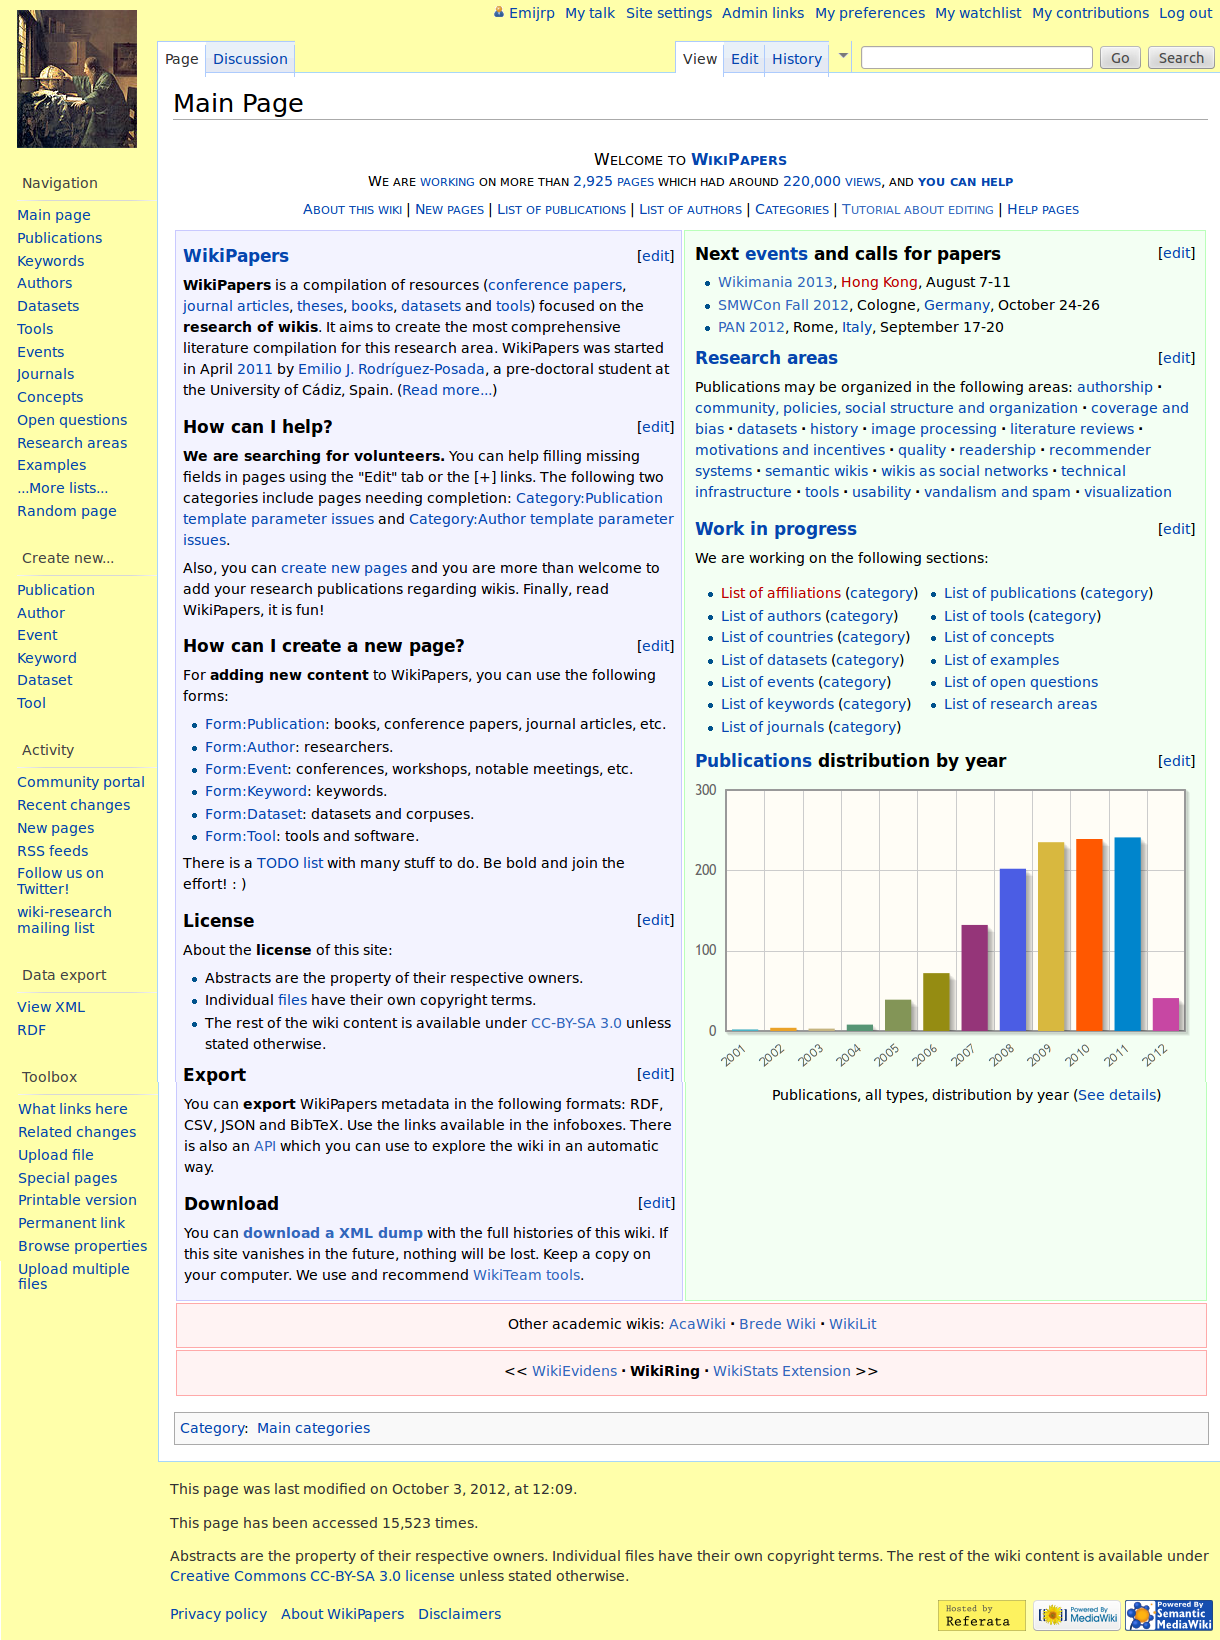
\includegraphics[width=0.8\textwidth]{wpfull.png}
\caption{Portada de WikiPapers}
\label{fig:wpfull}
\end{figure}


\section{Conclusiones y trabajo futuro}
porqué hacía falta WikiPapers
aglutina todas las ventajas de los anteriores sistemas
lo que se ha hecho, cifras,
lo que queda por hacer y como ayudar
el futuro y más allá...



\bibliographystyle{wink}        
\bibliography{proyecto-investigacion-2012}

\section*{Licencia}
Esta obra está bajo licencia \href{http://creativecommons.org/licenses/by-sa/3.0/}{Creative Commons Reconocimiento-CompartirIgual 3.0 Unported}.

\end{document}
